\section{Motivation}

Angular control in LIGO is an important contribution to the noise budget at the frequencies of highest sensitivity \cite{T0900511}. 

There are four different angular modes for the two Fabry-Perot arms in the LIGO interferometer, shown in figure \ref{fig:sidlessiggmodes}. 
The two hard modes are stable as the power increases, which means that the radiation pressure will push the mirrors back to an equilibrium position.
The two soft modes are unstable as the power increases, pushing the mirrors away from equilibrium. 
Despite being stable, the hard modes still exhibit a resonant behavior that will need to be damped.

\begin{figure}[htp]%
\includegraphics[width=.8\textwidth]{figures/application/SidlesSigg}%
\caption[Sidles-Sigg Modes]{The four Sidles-sigg modes of the Fabry-Perot cavities in LIGO. The two hard modes are stable and the two soft modes are unstable. All of modes must be damped with control loops.}%
\label{fig:sidlessiggmodes}%
\end{figure}

Angular noise can couple in to differential arm length (DARM) though the interaction between beam spot motion (BSM) and angular motion ($\theta$) on mirrors. This happens in two ways: both a static offset in the BSM with mirror angular noise and a static angular offset with BSM noise can create DARM noise. 

\begin{equation}
\hat{\Delta L}(f) = \hat{d}_{spot}(f)*\hat{\theta}_{Mirror}(f) \approx \hat{d}_{spot}(f)*\theta_{Mirror}^{RMS}(f) + d_{spot}^{RMS}(f)*\hat{\theta}_{Mirror}(f)
\label{eq:darmcouple}
\end{equation}

Barsotti and Evans showed that in Science Mode, angular noise from Common Soft and Differential Soft (the two modes of the arms that are unstable at high power) contribute the most to DARM noise. They also showed that in the final design of aLIGO, the soft mode is unstable with frequencies of -.17 and -.21 Hz for pitch and yaw, respectively. The control systems currently used for angular control must be used to damp the unstable modes and the resonances of the stable modes, which leads to injected sensing noise. For an optical angular control system to be useful, it must provide damping in that frequency range to stabilize the modes.

Using angular trapping methods, we can reduce the sensing noise injection by damping the angular motion $\hat{\theta}_{Mirror}(f)$.

\section{Applying angular control}

For our discussion, we will disregard the distinction between common and differential modes of the interferometer.

%I have considered two possible options that could (with some effort) be implemented in a LIGO-style interferometer.
%
%\subsection{Local damping}
%
%Damping relative to something very heavy in the end station. This is analogous to (and much harder than) just increasing the mass of the test mass.
%
%BSC4 layout: D0901154
%
%Pros:
%
%\begin{itemize}
	%\item Can keep the same ETM/ITM suspensions
	%\item Modular: easy to modify and/or disable
	%\item Easier to build, align and lock
	%\item Affects Soft and Hard modes equally.
%\end{itemize}
%
%Cons:
%\begin{itemize}
  %\item	Different parameters for ETM and ITM
	%\item Folded Cavities
	%\item worry about ISI weight limit
%\end{itemize}
%
%
%
%\begin{figure}[htp]%
%\begin{center}
%\includegraphics[width=.8\textwidth]{figures/application/shortTrapDiagram}%
%\caption[Local angular control]{Diagram of a local angular control scheme. This relies on the small mirrors being mounted in something heavier than the test mass.}%
%\label{fig:shorttrapdiagram}%
%\end{center}
%\end{figure}
%
%
%\begin{table}[htp]
%\centering
%\begin{tabular}{ l | l | }
%\bf{Parameter}& \bf{Metric}  \\ \hline
%Cavity length, $L$ & 2 m \\ \hline
%ETM power transmission, $T2$ & 5 ppm \\ \hline
%ETM $r2$ &0.9999975 \\ \hline
%ETM Diameter $D$ & 34 cm \\ \hline
%ETM Thickness $t$ & 20 cm \\ \hline
%Side diameter $D_s$ & 48 cm \\ \hline
%Side thickness $t_s$ & 30 cm \\ \hline
%Side ROC & 1.5 m \\ \hline
%Cavity $FSR$ & 75 MHz \\ \hline
%
%\end{tabular}
%\caption[Local angular design]{Characteristics of proposed local angular design}
%\label{tab:localproposal}
%\end{table}
%
%\begin{table}[htp]
%\centering
%\begin{tabular}{ l | l | }
%\bf{Parameter}& \bf{Metric}  \\ \hline
%Carrier Power $P_c$ & 10 W \\ \hline
%Subcarrier Power $P_s$ & 2 W \\ \hline
%Carrier Detuning $df_c$ & 9000 Hz \\ \hline
%Subcarrier Detuning $df_s$ & -2500 Hz \\ \hline
%OS Angle $\theta$ & 45 deg \\ \hline
%\end{tabular}
%\caption[Local angular optical springs]{Characteristics of proposed local angular optical spring}
%\label{tab:localos}
%\end{table}
%
%In this design, we use radiation pressure to couple e.g. the ETM (about 40 kg) to two much larger masses (about 400 kg each) made out of stainless steel. In this fashion, we can damp the angular motion of the test mass relative to the hopefully much more stable masses on the side. 
%
%With the control beams at \~ 45 degrees to the optical axis, we expect that the coating will be significantly lower reflectivity. Er-glass lasers at 1540 nm 
%
%\subsection{4 km damping}
%
%\begin{figure}[htp]%
%\begin{center}
%\includegraphics[width=.8\textwidth]{figures/application/longTrapDiagram}%
%\caption[4 km angular control]{Diagram of a 4km angular control scheme. This relies on control mirrors attached to the side of the test mass.}%
%\label{fig:longtrapdiagram}%
%\end{center}
%\end{figure}
%
%Damping ETM relative to ITM. This will have significant changes because the masses of the ETM and ITM are currently the same. The angular trap we have damps the motion of one mirror by pushing on the other. In a system with equal masses, this just couples the mirrors, it doesn't damp. 
%
%Pros:
%
%\begin{itemize}
	%\item Straight cavities
	%\item Lower vacuum chamber volume
	%\item Damp only Soft mode
%\end{itemize}
%
%Cons:
%\begin{itemize}
	%\item Does not see Hard mode motion of cavity
	%\item Modify test masses and probably suspensions
	%\item Hard/risky to adjust
%\end{itemize}
%
%
%\begin{table}[htp]
%\centering
%\begin{tabular}{ l | l | }
%\bf{Parameter}& \bf{Metric}  \\ \hline
%Cavity length, $L$ & 3994.5 m \\ \hline
%ITM power transmission, $T1$ & 1.4\% \\ \hline %T0900043

%ETM power transmission, $T2$ & 5 ppm \\ \hline
%ITM $r1$ & 0.99298 \\ \hline
%ETM $r2$ &0.9999975 \\ \hline
%Cavity $FSR$ & 37.52 kHz \\ \hline
%\end{tabular}
%\caption{Characteristics of proposed long angular design}
%\label{tab:longproposal}
%\end{table}
%
\subsection{Single spring 4km damping}

If we assume that the length will be stabilized with the main beam of the interferometer, we only really need to control the angular motion. We will consider only the yaw of the mirrors for this exploration, but there should not be any obstacles to applying the method to both pitch and yaw. 

It seems like we could do this with a single folded cavity (see fig \ref{fig:longtrapfoldeddiagram}). In this configuration, ETMs and ITMs would have `Buddy' mirrors attached to the sides to create an angular optical spring cavity.

This has several benefits that look quite appealing. The yaw of the ETM is damped relative to the ITM. If implemented ideally, the radiation pressure will be independent of small angular motions of the ETM. This particular configuration (see table \ref{tab:foldedos} has a UGF of about 8 Hz, so it should also damp the hard mode (Barsotti and Evans give a hard mode frequency of 3.05 Hz). This would also, as a byproduct, give a very sensitive readout of the yaw of the ETM via the PDH error signal.

There are several concerns that would need to be addressed. This configuration could actively couple angular noise in the ITM into length noise at the ETM. It would also require massive engineering changes to manufacture and align a monolithic test mass with Buddy mirrors bonded onto the sides. These mirrors would also need to be very carefully manufactured and attached, because the cavity could not be realigned once assembled.  

The design has to be careful of losses due to long-storage-time optical cavities\cite{Isogai13}, but the finesse is low enough in this configuration ($F=7850$) to avoid a significant impact from the effects. The design also has the potential to introduce increased thermal noise to the length degree of freedom, due to the added buddy mirrors. We have neglected the thermal noise effects in this analysis, but it should be addressed.


\begin{table}[htp]
\centering
\begin{tabular}{ l | l | }
\bf{Parameter}& \bf{Metric}  \\ \hline
Cavity round-trip length, $4L$ & 16 Km \\ \hline
Buddy Mirror power transmission, T1,T2 & 200 ppm \\ \hline
Buddy Mirror power absorption, T1, T2 & 2 ppm \\ \hline
Buddy Diameter $D$ & 15 cm \\ \hline
Buddy Thickness $t$ & 10 cm \\ \hline
Buddy ROC & 3.5 km \\ \hline
Cavity $FSR$ & 18.7  kHz \\ \hline
Cavity Finesse & 7850 \\ \hline

\end{tabular}
\caption[Folded angular design]{Characteristics of proposed angular design. The transmissivity and absorption values are easily achievable with current dielectric coatings.}
\label{tab:foldedproposal}
\end{table}

\begin{table}[htp]
\centering
\begin{tabular}{ l | l | }
\bf{Parameter}& \bf{Metric}  \\ \hline
Carrier input power $P_c$ & 6 W \\ \hline
Subcarrier input power $P_s$ & .15 W \\ \hline
Carrier Detuning $df_c$ & 19 Hz \\ \hline
Subcarrier Detuning $df_s$ & -5 Hz \\ \hline
OS Angle $\theta$ & 62.5 $\mu rad$ \\ \hline
OLG UGF & 7.9 Hz \\ \hline
Phase at UGF & -169.3 deg \\ \hline
\end{tabular}
\caption[Folded angular optical springs]{Characteristics of proposed angular optical spring. The relatively low power (about 6 watts) is easily achievable. The detunings will require careful design because they are very small.}
\label{tab:foldedos}
\end{table}

Table \ref{tab:foldedos} lists the parameters for a possible optical spring design. If we lock the laser to the frequency of the main cavity laser, we can take advantage of the fantastic frequency stabilization of a 4 km cavity, and also remove the common mode length noise of associated with relative frequency fluctuations. The very small frequency detunings would still present a significant challenge to implement and maintain.

\begin{figure}[htp]%
\begin{center}
\includegraphics[width=.6\textwidth]{figures/application/longFoldedDiagram}%
\caption[4 km angular control]{Diagram of a folded cavity 4km angular control scheme. This configuration relies on `Buddy' mirrors attached to the side of the test masses.}%
\label{fig:longtrapfoldeddiagram}%
\end{center}
\end{figure}

\begin{figure}[htp]%
\begin{center}
\includegraphics[width=\textwidth]{figures/application/OLG}%
\caption[4 km angular open loop gain]{Open loop gain ($OLG$) of the angular control scheme and optical springs. The optical springs shown are the carrier and subcarrier optical spring constants ($KOS_C$ and $KOS_S$) and the total optical spring ($KOS_T$).}%
\label{fig:longtrapfoldedOLG}%
\end{center}
\end{figure}

\begin{figure}[htp]%
\begin{center}
\includegraphics[width=\textwidth]{figures/application/SAF}%
\caption[4 km angular closed loop gain]{The actuation function ($ACF$) and spring actuation function ($SAF = CLG\times ACF$) of the proposed angular control scheme. The actuation function includes the yaw pendulum behavior ($1/f^2$) of the mass and the yaw resonant frequency (chosen to be 0.5 Hz) of the ETM. }%
\label{fig:longtrapfoldedSAF}%
\end{center}
\end{figure}



%\section{noise benefits}
%
%The cool thing about this method is that it can work independently and in tandem with existing control systems. 

%\section{path to angular damping with optical springs in aLIGO}
%
%I think we might want to get rid of this section.